\documentclass{article}

\usepackage{amsmath}
\usepackage{amssymb}
\usepackage{parskip}
\usepackage{fullpage}
\usepackage{hyperref}
\usepackage{blkarray}
\usepackage{tikz}

\hypersetup{
    colorlinks=true,
    linkcolor=black,
    urlcolor=blue,
    pdftitle={Graphs},
    pdfpagemode=FullScreen,
}

\title{Graphs}
\author{Paolo Bettelini}
\date{}

\begin{document}

\maketitle
\tableofcontents
\pagebreak

\section{Adjacency Matrices}

A finite graph can be represented by a square matrix
\(n \times n\) where \(n\) is the number of vertices.

\begin{center}
    \begin{minipage}[r]{6cm}
        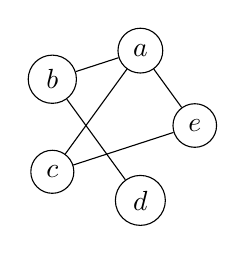
\begin{tikzpicture}[main/.style = {draw, circle}]
            \foreach \x [count = \xi] in {a,b,c,d,e} {
                \node[main] (\xi) at
                    ({1 * cos(360 / 5 * \xi)}, {1 * sin(360 / 5 * \xi)})
                    {\(\x\)};
            }
        
            \draw (1) -- (2);
            \draw (1) -- (3);
            \draw (1) -- (5);
            \draw (2) -- (4);
            \draw (5) -- (3);
        \end{tikzpicture} 
    \end{minipage}
    \begin{minipage}[l]{6cm}
        A=
        \begin{blockarray}{cccccc}
            & a & b & c & d & e \\
            \begin{block}{c(ccccc)}
            a & 0 & 1 & 1 & 0 & 1 \\
            b & 1 & 0 & 0 & 1 & 0 \\
            c & 1 & 0 & 0 & 0 & 1 \\
            d & 0 & 1 & 0 & 0 & 0 \\
            e & 1 & 0 & 1 & 0 & 0 \\
            \end{block}
        \end{blockarray}
    \end{minipage}
\end{center}

Every row and column represents a vertice. \(1\) means
that the two vertices are adjacent, \(0\) otherwise. The diagonal of this matrix
will always e \(0s\) since no vertice is adjacent to itself
and \(A=A^t\)

\end{document}
